\section{Komponenten Optimierer Prototypen}




\begin{figure}[ht]
  \centering
  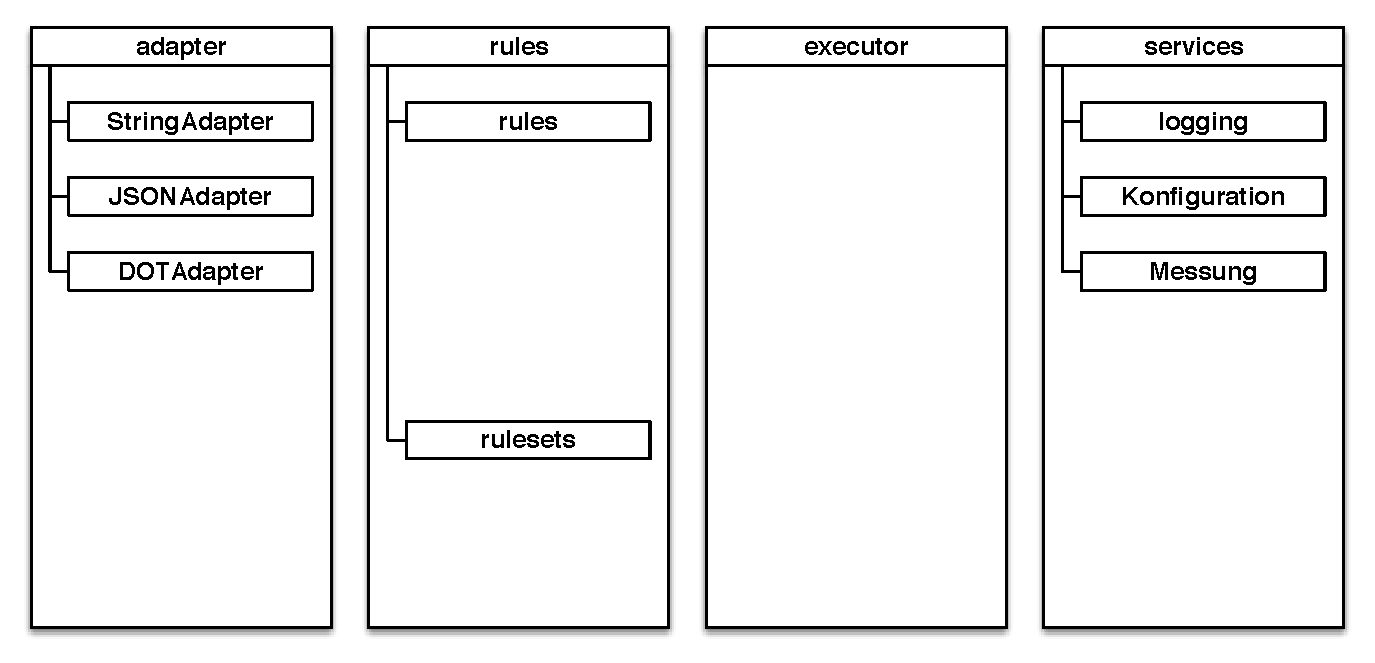
\includegraphics[width=\textwidth]{04_Implementierung/Organization.pdf}
  \caption{Projektorganisation}
  \label{ProjectOrga}
\end{figure}


Das Projekt ist entlang der unterschiedlichen Aufgaben modular organisiert. Unter dem Dach der Anwendung finden sich vier unterschiedliche Sparten, die gemeinsam für das Ausführen des Programms verantwortlich sind: Planknoten und Äuqivalenzklassen, Regeln und Regelmengen, Ineratoren und Services. Die genaue Zuordnung zu den jeweiligen Bereichen ist in Abb. \ref{ProjectOrga} nachvollziehbar.




Bei der Ausführung eines Tests  müssen alle Bereiche zusammenarbeiten. Der Service-Bereich und insbesondere das Konfigurationsmodul sind für die konkrete Zusammenstellung der für den Test notwendigen Komponenten verantwortlich. Er entscheidet, welche Regeln zum Einsatz kommen, welcher Enumerator gewählt wird, welche konkreten Pläne getestet und mit Hilfe welcher Adapter die Daten ein-  bzw. ausgegeben werden. Um zu verstehen, welche Möglichkeiten das implementierte System bietet, sind die einzelnen Komponenten im Folgenden im Detail beschrieben.


\subsection{Services}
Da für die Ausführung des Programms unterschiedliche Dienstleistungen benötigt werden, die auch in anderen Kontexten relevant sein können, falls das Projekt diese Funktionen im Bereich Services zusammen. Teil des Bereichs ist der Konfigurator, der die Konfiguration der Tests übernimmt, die Zeitmessung und Das Logging von Informationen.

Nicht alle Komponenten wurden selbst entwickelt, beispielsweise wurde beim Logging auf die existierende Library \texttt{easylogging++} gesetzt. Auch für das Parsen von JSON-Files ist die externe Bibliothek json11 verwendet worden.



\subsubsection{Konfiguration}


\begin{figure}[ht]
  \centering
  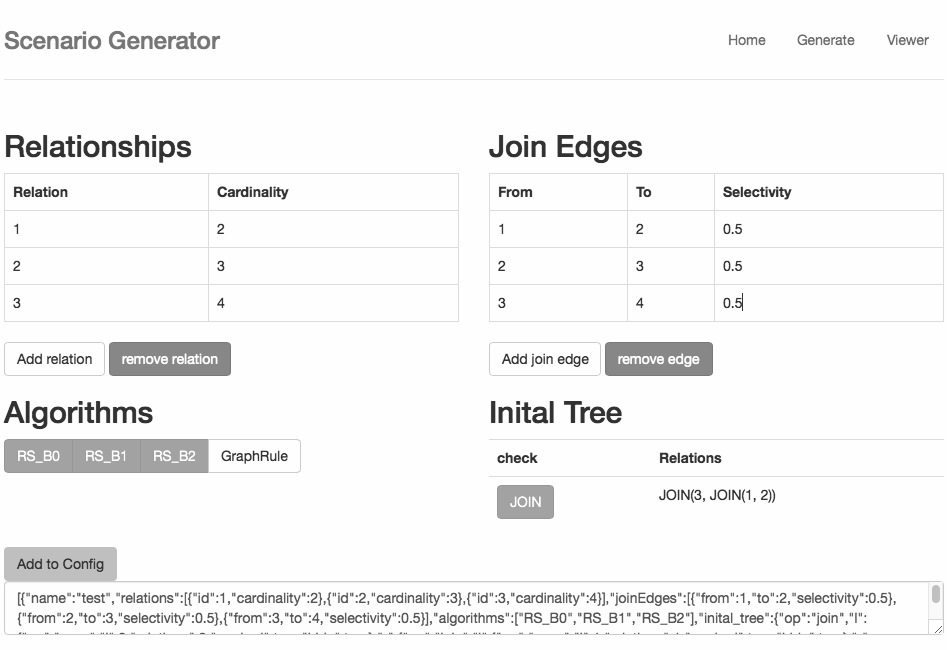
\includegraphics[width=1\textwidth]{04_Implementierung/Tool.png}
  \caption{Konfigurationstool: Scenario-Generator}
  \label{ScenarioGenerator}
\end{figure}

Das Konfigurationsmodul besteht aus zwei Komponenten. Auf der einen Seite eine Javascript-HTML Anwendung zur Generierung von Test-Szenarien (vgl. Abb. \ref{ScenarioGenerator}). Mit Hilfe dieser Anwendung können Konfigurationsfiles für den späteren Test erstellt werden. Dieses Konfigurationssystem, das in  zu sehen ist, bietet dem Nutzer die Möglichkeit Relationen mit Kardinalitäten zu erzeugen, Selektivitäten festzulegen und schlussendlich einen initialen Plan zu erzeugen. Ebenfalls ist es möglich die verschiedenen Regelmengen, die geprüft werden sollen, festzulegen.
Das Ergebnis dieses Moduls ist eine Konfigurationsdatei im JSON-Format. Das Tool unterstützt die Erzeugung mehrerer Szenarios in einem Konfigurationsfile. So können mehrere Szenarios in einem Test-Run durchgespielt werden. Die Verwendung des JSON-Formats bietet viele Vorteile:

\begin{itemize}
\item Neue Felder können in der Datei angefügt werden, so ist es möglich leicht neue Attribute und Objekte dem Konfigurationsfile hinzuzufügen.
\item JSON ist ein standardisiertes Format.
\item 
\end{itemize}

Ein konkretes Test File ist in \ref{JsonConfigFile} zu sehen. Jedes Test File ist ein Array von Test-Objekten. Für jeden Test wird mit dem Attribut \texttt{name} ein Name gespeichert. Für jede Relation, die in einem Test vorkommt, wird ein Relations-Objekt erzeugt. Es besteht aus einer \texttt{id}, der Relations-Id, und der dazugehörigen Kardinalität. Mehrere dieser Relations-Objekte werden in einem Array gespeichert und sind dem \texttt{relation}-Attribut des Test-Objekts zugewiesen. Im Konkreten Fall sind zwei Relationen vorhanden. Eine mit der \texttt{id:1} und eine mit der \texttt{id:2} 2. Für beide wurde eine Kardinalität zugewiesen. 

Auch für Join-Kanten werden Objekte erzeugt. Ein Join-Kanten Objekt bezeichnet eine Kante zwischen zwei Relationen. Eine Kante könnte, wie im Beispiel zu sehen von der Relation 1 zu der Relation 2 verlaufen, wobei die Richtung nicht entscheidend ist. Einer Join-Kante wird auch eine Selektivität zugeordnet. Mehrere dieser Join-Edge-Objekte werden als Array im Attribut \texttt{joinEdges} hinterlegt.

Neben Join-Kanten und Relationen sind auch die zu testendeden Algorithmen gespeichert. Sie werden in einem Array abgelegt und sind dem Attribut \texttt{algorithms} zugewiesen. Im vorliegenden Beispiel werden die Regelsets \texttt{RS-B0}, \texttt{RS-B1} und \texttt{RS-B2} getestet.

Auch ein initialer Plan wird im Test-Objekt gespeichert. Ein Baum besteht immer aus Knoten. Für jeden Knoten wird ein Operator im Attribut \texttt{op} gespeichert. Es wird der Operator \texttt{SCAN} und der Operator \texttt{JOIN} unterstützt. Ein Knoten kann eine linke und eine rechte Seite haben. In Zeile 14 ist eine Scan Operation zu sehen. Es wird nur die linke Seite verwendet. Im Attribut \texttt{l} ist die ID der Relation abgelegt, die zu scannen ist. Bei \texttt{JOINs} wird auch die rechte Seite verwendet (vgl. Zeile 16). In den Attributen \texttt{l} und \texttt{r} können entweder weitere Knoten oder Relations-Ids gespeichert werden. Neben Operator, links und rechts ist das Attribut \texttt{relations} Teil des Knotens. hier ist eine einfache Repräsentation des Knotens gespeichert. Im Falle von Zeite 14 \texttt{1}. Sind komplexere Knoten und Subknoten vorhanden, können komplexere Daten im Feld \texttt{Relations} abgelegt sein. Beispielsweise ist eine solche komplexere Form in Zeile 19 ( \texttt{JOIN(1,2)}) zu erkennen. Hier ist ein Join zwischen 1 und 2 zu sehen.

\begin{minipage}{\linewidth}

\linespread{0.5}\lstinputlisting[caption=Konfigurations-File, label=JsonConfigFile]{04_Implementierung/config.json}
\end{minipage}


Die eigentliche Konfiguration findet in C++ statt. Mit der Bibliothek json11 \cite{json11} wird das Konfigurationsfile gelesen. Für jedes Szenario und jede Regelmenge wird ein initaler Baum aus Äquivalenzklassen und Planknoten mit einem JSON-Adapter gebildet. Der Exekutor wird gewählt und mit einer Regelmenge initialisiert. Der initiale Baum wird dem Exekutor übergeben. Nachdem die Regeln angewendet wurden, startet der Konfigurator die Kostenschätzung. Nachdem alle Szenarios abgearbeitet sind, ist das Programm beendet.

\subsubsection{Zeitmessung}

\begin{figure}[ht]
  \centering
  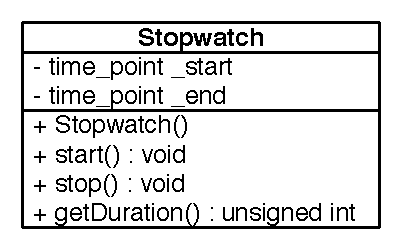
\includegraphics{04_Implementierung/Stopwatch.pdf}
  \caption{Klassendiagramm: Stopwatch}
  \label{ClassStopwatch}
\end{figure}

Wie bereits in Abb. \ref{Ablauf} dargestellt, wird die Zeitmessung, die durch die Klasse Stopwatch (vgl. Abb. \ref{ClassStopwatch}) durchgeführt wird, nach der Konfiguration zuerst instantiiert und dann mit der Methode \texttt{start()} gestartet. Sobald alle Pläne expandiert und die Kosten berechnet sind, wird die Messung durch die Methode \texttt{stop()} beendet. Um eine möglichst genaue Messung durchführen zu können, wurde die Uhr \texttt{std::chrono::steady\_clock} verwendet. Diese Uhr ist Teil von C++11. Wie in der Dokumentation \cite{cppreference_2015_clock} beschrieben, handelt es sich bei der Uhr um eine monotone Uhr. Sie kann nicht rückwärts laufen, solange die physische Zeit fortfährt. Die Uhr selbst mit der Wall\-Clock\-Time verbunden ist das passende Werkzeug zur Messung von Intervallen. 

Die Dauer zwischen Start der Expansion und dem Ende der Kostenberechnung wird in Nanosekunden gemessen und mit der Methode \texttt{getDuration()} ausgegeben, um ein möglichst akkurates Ergebnis zu erhalten. Die gemessenen Ergebnisse werden sowohl als Debug-Log in der Konsole ausgegeben,als auch  in einem Log File gespeichert.




\subsubsection{Logging und Debugging}
Zum Debugging wurde auch eine externe Bibliothek eingesetzt: EasyLogging++ \cite{easylogging}, ein einfach zu bedienendes, jedoch hochgradig konfigurierbares Logging Instrument. Gerade die Leichtgewichtigkeit - das Tool besteht nur aus einer Headerklasse -, die einfache Bedienung und die Geschwindigkeit gaben  den Ausschlag zur Nutzung der Library. Mit Hilfe dieser Library werden debugging Informationen geschrieben, aber auch Zeitmessungen gespeichert, Pläne ausgegeben und sonstige Debugging Nachrichten ausgegeben. Insbesondere ist die Unterscheidung zwischen unterschiedlichen Debug\-Leveln wichtig. Auf mehreren Ebenen (INFO, WARNING, DEBUG, etc.) können Informationen ausgegeben werden. Je nachdem welches Level angesprochen ist, werden nur Informationen über dieses ausgegeben. 


\subsection{Adapter}

Die Implementierung bietet mehrere Adapter, die zur Umwandlung von externen Formaten in eine interne Repräsentationsform, oder von einer internen Repräsentationsform in ein externes Format genutzt werden können. Sie bieten die Möglichkeit andere Systeme an das bestehende System anzudocken und sorgen so für den notwendigen Anschluss und die Erweiterbarkeit durch Dritte.

Insgesamt werden drei Adapter mitgeliefert. (1) JSON\-Adapter, (2) String\-Adapter, (3) DOT\-Adapter.

Der Json-Adapter erlaubt es Daten im JSON Format zu importieren und wird beim Einlesen des initalen Plans genutzt. Er wandelt auf der Basis des Konfigurationsfiles JSON in Planknoten und Äquivalenzklassen um, die dann weiterverarbeitet werden können. Ebenfalls ist es möglich, Pläne in JSON auszugeben. Zu diesem Zweck implementiert der Parser auch eine \texttt{dump} Methode.

Neben dem JSON\-Adapter wird auch ein String Adapter verwendet. Er ist für die Ausgabe von Plänen als String verantwortlich. Im Gegensatz zu einem JSON\-Adapter ist die Eingabe von Plänen mit Hilfe dieses Moduls nicht möglich. Auch der DOT\-Adapter erlaubt nur die Ausgabe von Plänen im DOT\-Format, die  zur Generierung von graphischen Ausgaben verwendet werden können.

Eine weitere Aufgabe eines solchen Adapters kann auch die Übersetzung von Relationsnamen in Bitvektoren sein. Da das vorliegende System, wie in \ref{sec:Bitvector} beschrieben, Relationen als Bitvektoren abbildet, mag es nützlich sein, Relationsnamen in Bitvektoren zu übersetzen. Für diese Übersetzung sind auch Adapter vorgesehen, die zusätzlich implementiert werden können.












\subsubsection{Erweiterbarkeit von Regelsets}





\subsubsection{Ausführung von Regeln}

Das eigentliche Ausführen der Regeln wird durch einen XY durchgeführt. Im konkreten Fall kommt hier der Algorithmus ExhaustiveTransformation zum Einsatz. Der Algorithmus startet mit einer Äquivalenzklasse. Innerhalb dieser Äquivalenzklasse werden die Regeln, die durch ein Regelset vorgegeben sind auf einem PlanKnoten ausgeführt. Die Ausführung geschieht hierbei zuerst auf den Oberen Ebenen und setzt sich dann auf den Kindern eines Knoten fort. Somit können bei der Transformation eines gegebenen Baums alle Regeln auf andere Bäume angewendet werden.

Wichtig ist hierbei zu bemerken, dass dieser Algorithmus immer zuerst prüft, ob eine Regel auch tatsächlich für die Anwendung geeignet ist und dann erst der Algorithmus ausgeführt wird. Neben der eigentlichen Eignung wird auch geprüft, ob eine Äquivalenzklasse bereits vollständig expandiert wurde. Falls dies der Fall ist, wird von einer weiteren Anwendung von Regeln abgesehen. Diese Funktion kann insbesondere Vorteile bei der Implementierung von neuen Regelsets bieten. Nutzt ein gegebenes Regelset die Möglichkeit nicht nur einen neuen Planknoten zu generieren, sondern gleich mehrere Planknoten zu erstellen und auch in diesem Zusammenhang bereits mehrere Kinder-Knoten zu erstellen, kann die Reihenfolge der Expansion von Äuqivalenzklassen geändert werden. Die einzelnen Äquivalenzklassen, die bereits durch eine Regel expandiert wurden, werden als solche markiert und die bisher vorhandenen Regeln werden nicht mehr ausgeführt.




\subsection{Relationen, Planknoten und Äquivalenzklassen}




\subsubsection{Planknoten und Äquivalenzklassen}




\subsubsection{Konkrete Implementierung}

Die konkrete Implementierung der Äquivalenzklasse sieht vor, wie in Abb. \ref{EquivalenceClassDiagram} zu erkennen, dass für jede Äquivalenzklasse die darin aggregierten Relationen, sowie deren Nachbarn gespeichert werden. Ebenfalls wird der erste, letzte und kosteneffektivste Planknoten gespeichert. Außerdem kann festgehalten werden, ob eine Äquivalenzklasse bereits $explored$, also erforscht, ist. 






\subsubsection{Enumeratoren}





















\subsubsection{Erweiterbarkeit von Regeln}

Die Erweiterbarkeit ist auf mehreren Ebenen sichergestellt. Auf der einen Seite können neue Regeln erzeugt werden. Sobald diese die Form der abstrakten Klasse $Rule$ übernehmen, können sie in Regelsets zum Einsatz kommen. Ein Beispiel für eine solche Erweiterung ist die Regel $GraphRule$. Sie wurde später der entwickelten Lösung hinzugefügt. Die neue Regelmenge $GraphRuleSet$ beinhaltet in diesem speziellen Fall nur eine Regel.

Eine weitere Möglichkeit zur Erweiterung wurde ebenfalls von $GraphRule$ genutzt. GraphRule gibt nicht nur einen einzelnen neuen Planknoten zurück, sondern übergibt gleich einen vollständig expandierten Baum. Auch diese Anforderung konnte ohne Veränderung des Interfaces umgesetzt werden. Da der Planknoten ein $next$ Attribut besitzt, das den vorhergehenden mit dem nächsten Knoten verbindet, können Ketten von neuen Knoten gebildet werden. Diese Ketten werden im Falle der $GraphRule$ zurückgegeben ohne dabei das Interface zu brechen.

Neben den vorgegebenen  Methoden können auch weitere Methoden für eine Regel implementiert werden. Dies ist beispielsweise bei $GraphRule$ notwendig gewesen. Hier ist es erforderlich, dass der Graph zuerst partitioniert wird, dann ConnectedComponents gefunden und schlussendlich ein Baum zurückgegeben wird. Auch dies ist innerhalb der Rules möglich.

Eine weitere Möglichkeit zur Erweiterung ist durch Templates gegeben. Template ist eine Funktion von C++ mit deren Hilfe Funktionen und Klassen mit generischen Typen arbeiten können. Dadurch ist es einer Funktion der einen Klasse möglich, viele unterschiedliche Typen zu unterstützen, ohne die Funktion oder die Klasse bearbeiten zu müssen. Im konkreten Fall der Regeln werden zwei dieser generischen Typen verwendet: $PlanNode$ und $Operations$. Es wird somit möglich, die Klassen des Planknotens und die möglichen Operationen, die für diese Planknoten möglich sind zu ersetzen, ohne Funktionen und Klassen verändern zu können.



\subsection{Kostenschätzung und statistische Informationen}



Die Kostenschätzung zur Suche des optimalen Plans geschieht bei der vorliegenden Implementierung in einem eigenen Kostenschätzungsmodul.Teil des Kostenmoduls ist ein Katalog innerhalb dessen Informationen über Selektivität von JOINs und Kardinalitäten von Relationen gespeichert sind. Diese Informationen werden aus dem Katalog mit Hilfe des Kostenschätzers ausgelesen und die Kosten für einen Planknoten berechnet.

Die Berechnung der Kardinalität findet bottom up statt. Für jede Äquivalenzklasse wird die optimale Kardinalität berechnet und gespeichert. Der Planknoten mit dessen Hilfe diese optimale Kardinalität erreicht wird, wird als bester Planknoten markiert. Folgt man dem Pfad der besten Planknoten ergibt sich der kostenoptimale Baum an Planknoten. Die Berechnung sieht vor, dass immer die Selektivität eines Operators mit dem Produkt der Kardinalität der Eingabeparameter multipliziert wird. Beispielsweise wird auf der untersten Ebene - der Ebene der Scans - für eine gegebene Relation die Kardinalität mit der Selektivität von 1 multipliziert, da die gesamte Relation verarbeitet werden muss. Bei einem Join können komplexere Situationen auftreten. Zuerst wird das Produkt der Kardinalität der Eingabe Parameter berechnet. Diese kann dann mit der 
Selektivität multipliziert werden. Das Produkt der Kardinalitäten repräsentiert in diesem Falle die Kardinalität des möglichen Kreuzproduktes, das mit Hilfe von Selektoren eingeschränkt wird.



\subsection{Zusammenfassung}

Gerade im Bereich der Regeln ist klar zu erkennen, dass die SOLID Prinzipien eingehalten wurden. Hier ist jede Klasse nur für genau eine Aufgabe zuständig. Ein hohes Maß an Kohäsion konnte erreicht werden. Die Regelklassen  sind offen für Erweiterungen, jedoch geschlossen für Modifikationen. Dies wird insbesondere bei der Erweiterung mit Hilfe des Regelsets $GraphRuleSet$ deutlich. Auch das Liskov Substitutionsprinzip wurde eingehalten. Alle Klassen verhalten sich nach außen gleich und liefern dasselbe Ergebnis, einen Planknoten, zurück. 